\documentclass[conference,9pt]{IEEEtran}
\usepackage{xcolor}
\usepackage{cite}
\usepackage{epsfig}
\usepackage{amssymb}
\usepackage{amsmath}
\usepackage{graphicx}
\graphicspath{ {./} }

\begin{document}
\title{Practical 3}

\author{
\IEEEauthorblockN{Albert Acebron}
\IEEEauthorblockA{NIU: 1458626}
}


% make the title area
\maketitle
\begin{abstract}
This practical will be based on an analysis of a GNSS sinal and another one that has been distorted by third one. To do that we'll study several estimation methods based on Power Spectrum Density, apply them, evaluate their results and compare them against each other.
\end{abstract}

\section{Introduction}
We'll start our study on PDS estimation with the periodogram, a non-parametric estimator, which we will use to identify the signal that we are looking for, and then we'll move on to parametric estimators. Afterwards we'll deepen our understanding of these estimators and proceed to analyse their properties under the scenario of recovering a GNSS signal. 

\section{Periodogram}

Let's put ourselves in the shoes of an engineer that has received a signal that is the result of adding two different ones, the signal that he's interested in and one that is interferring with it. To fix this signal up, one must start by finding out what signal are contained in it and how each one of these is, and to do so a good way to start is by using the periodogram of the received signal, since that allows us to estimate how the power density of that signal is distributed accross the spectrum.

To compute it we'll take its definition and convert it into an equivalent one that makes use of the fourier transform (this is a well known procedure so we'll skip over it here), which allows us to implement it with the following code:
\begin{verbatim}
  function S_per = compute_periodogram(signal)
    n=length(signal);
    S_per=abs(fft(signal)).^2/n;
  end
\end{verbatim}

Now we can proceed to apply it to our signal, but, before doing that let's do some calculations to make sure that the normalized resolution of our result is equal to a number we feel comfortable with, such as 0.0002.

To calculate the periodogram we are using a same-size DFT, and this means that the resulting vector will be on the frequency range from Fs/N to the sampling frequency (10MHz in this case), with a number of bins equal to the number of samples that were used to create the periodogram.

This means that the resolution of our result will be $\frac{10MHz}{N}$, but if we were to normalize the frequencies (so they go from 0 to 1 instead) this would become $\frac{1}{N}$. With this equation we can obtain the number of samples needed to achieve a resolution of 0.0002 by simply solving the following equation.
$$\frac{1}{N}=0.0002$$

Which yields the result:
$$N=\frac{1}{0.0002}=5000$$

The result of computing our periodogram (of a signal without noise) with that amount of samples from our signal is the following:

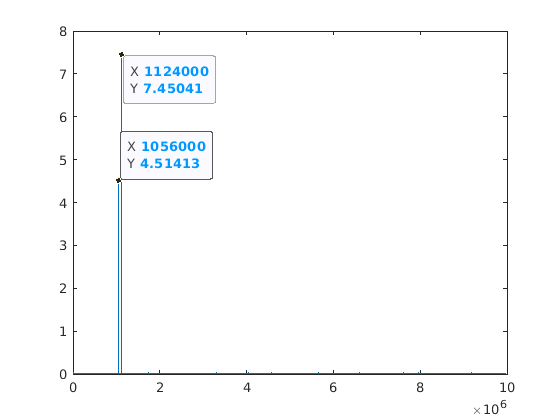
\includegraphics[scale=0.6]{q4}
\begin{verbatim}
  for p=[10, 100, 1000]
    N=5000;
    Px=compute_AR(RxSignal(1:N), p);
    Px=Px.*(max(abs(RxSignal(1:N)))/max(Px));
    x=Fs/N:Fs/N:Fs;
    plot(x, Px)
  end
\end{verbatim}
As shown on the figure, the estimated frequencies of the two signals that are contained within it are clearly 1.056MHz and 1.124MHz. As the practical states that interfering signal has a higher power, we can easily tell that our signal of interest will be the one located on 1.056MHz, as it's spectral power density is lower.

Now let's see how the number of samples used affects the results we are getting by applying the periodogram to our sinal with different amounts of samples ($10\mu s, 100\mu s, 500\mu s$) to see how it reacts to different resolution settings.

Given that the sampling frequency is 10MHz, a segment of length $m \mu s$ will be contained in $10^{6-6+1}*m$ discrete samples, which means that, to analyze segments of lengths $10\mu s, 100\mu s, 500\mu s$, we will use 100, 1000 and 5000 samples respectively.

Next we will take these segments and calculate their periodogram, get the two peaks/maximums contained within them and convert these to frequency values\footnote{Due to the fact that the periodogram covers the frequencies from 10MHz/N to 10MHz (the sampling freq), the bins will have a size of $\frac{10MHz}{N}$ where N is the number of samples used} with the following code:

The resulting estimated frequencies are:
\begin{center}
  \begin{tabular}{ c c c c c c c c c c }
    Length & First freq & Second freq \\
    $10\mu s$ & 1.2MHz & 1.1MHz \\
    $100\mu s$ & 1.13MHz & 1.07MHz \\
    $500\mu s$ & 1.126MHz & 1.058MHz \\ 
  \end{tabular}
\end{center}

As we can appreciate, an increase of the number of samples used gets us a higher precision in our results, enabling us to make better predictions of where are the two signals located in the frequency spectrum. This makes sense since the more samples we use the more data is available and the better our estimations can work.

Nevertheless, all our of results so far have been based on operating on a signal with no noise, something which doesn't mirror the effects that we would see in the real world. To step our game up, we'll need to start using a noisy signal, which will have a periodogram like this:

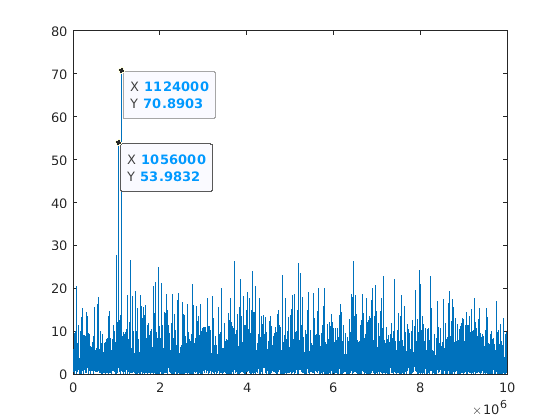
\includegraphics[scale=0.6]{q5}

Compared with the previous graph provided, in the spectrum of this signal we see much more noise across the spectrum but we can still clearly make out two peaks at 1.056MHz and 1.124MHz, which are the frequencies we are looking for. Therefore, in this case noise hasn't really been a problem in detecting the frequencies.

\section{AR estimator}
Let's look at another kind of estimator now, one based on fitting our signal to a autoregressive model. Contrary to the periodogram, this estimator is parametric, which means that we must provide a parameter (in this case $p$) for it to work, which requires some knowledge of the signal and the conditions in which it is received.

To begin playing with it first we'll present an implementation of it on matlab based on the formulas that were provided in the practical:

\subsection{Implementation}
We'll begin by estimating the biased autocorrelation using the xcorr function from Matlab (xcorr's also provides the negative values of the correlation so to get the it to start at x=0 we'll remove the first half of the results):
\begin{verbatim}
  rx=xcorr(signal, 'biased');
  rx=rx(N:end);
\end{verbatim}

Then let's construct the matrixes:
\begin{verbatim}
  r=rx(2:p+1);
  R=toeplitz(rx(1:p), conj(rx(1:p)));
\end{verbatim}

Solve for $a$ and $\sigma_w$:
\begin{verbatim}
  ar=-inv(R)*r;
  a=[1; ar];
  sigma=rx(1)+ar'*r
\end{verbatim}

The resulting sigma is $2.0108e+04 + 2.2737e-13i$, which should be a real number, but as we can see, it's a complex one. However, the complex part of the number is extremely insignificant compared to the real one (concretely, there's 17 magnitudes of difference between them) so we'll assume it's a numerical calculation error and eliminate it:
\begin{verbatim}
  sigma=real(sigma); % Remove numerical error
\end{verbatim}

And construct the final result:
\begin{verbatim}
  Sx=sigma./(abs(fft(a)).^2)
\end{verbatim}

This is already a correct implementation of the estimator, but, to get the same number of points in our results that the periodogram from before has, which will make comparisons easier, we'll compute the fft with N points:
\begin{verbatim}
  Sx=sigma./(abs(fft(a, N)).^2)
\end{verbatim}

Putting it all together:
\begin{verbatim}
function S_AR = compute_AR(signal, p)
  N=length(signal);
  rx=xcorr(signal, 'biased');
  rx=rx(N:end);
  r=rx(2:p+1);
  R=toeplitz(rx(1:p), conj(rx(1:p)));
  ar=-inv(R)*r;
  a=[1; ar];
  sigma=rx(1)+ar'*r;
  sigma=real(sigma); % Remove numerical error
  S_AR=sigma./(abs(fft(a, N)).^2);
end
\end{verbatim}

Let's now test it on our signal (first without noise) with different values for $p$:

Plot for $p=10$:

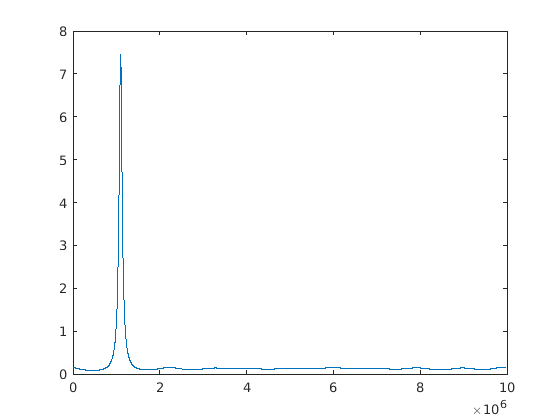
\includegraphics[scale=0.6]{p10}

Plot for $p=100$:

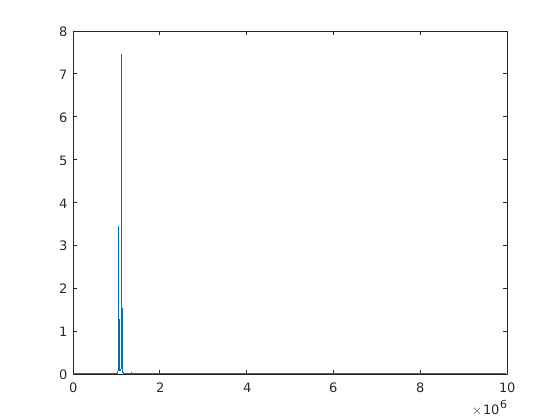
\includegraphics[scale=0.6]{p100}

Plot for $p=1000$:

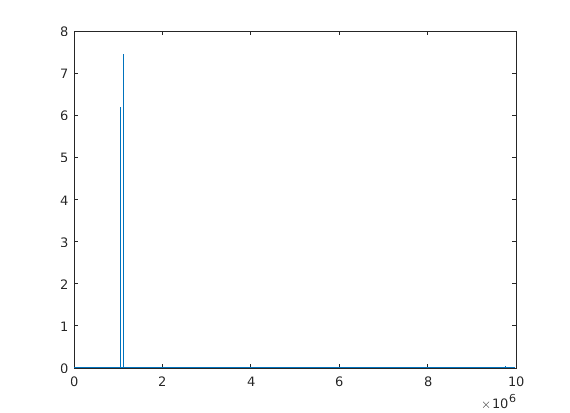
\includegraphics[scale=0.6]{p1000}

Observing these we appreciate that the plot where $p=1000$ is almost equal to the periodogram we computed earlier, whereas the one where $p=10$ resembles it a bit but is quite different and it's not possible to make out the two peaks, as they kind of get absorbed into a single peak. The plot made with $p=100$ is in the middle of these two: it's quite similar to the periodogram but not as much as the $p=1000$ plot.

In conclusion, the higher the value of $p$ (more concretely, the closer it is to $N$ the better), the closer the plot resembles the one we got in the previous section. 

If we now perform the same actions to a signal with AWGN noise (the same one we used before for our noisy periodogram), we get the following plots:

Plot for $p=10$:

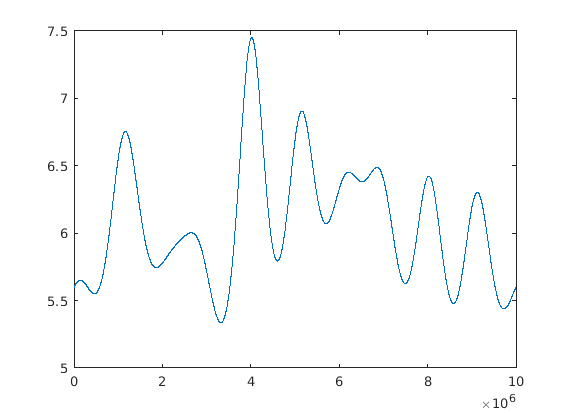
\includegraphics[scale=0.6]{pn10}

Plot for $p=100$:

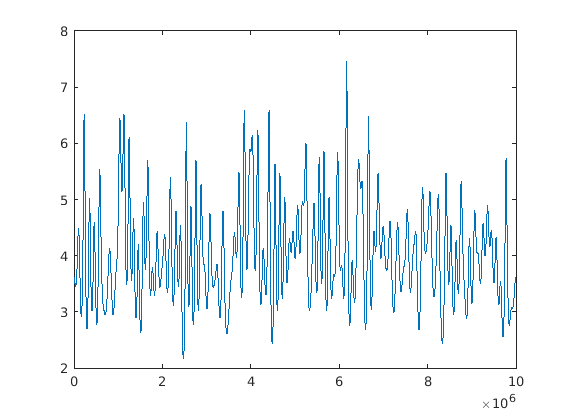
\includegraphics[scale=0.6]{pn100}

Plot for $p=1000$:

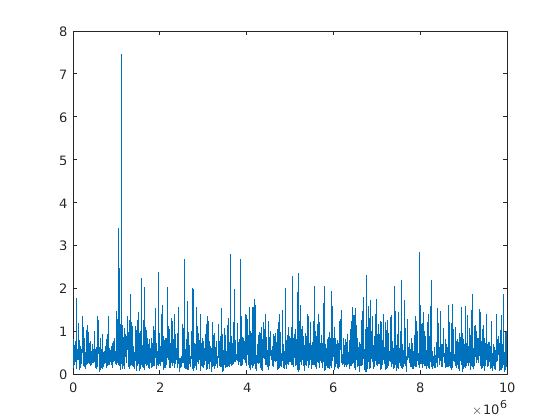
\includegraphics[scale=0.6]{pn1000}

In these graphs we can appreciate that graphs for $p=10$ and $p=100$ are completely different (this is because for low values of $p$ the autoregressive model used to estimate the signal isn't calculated properly when there's noise) whereas the graph for $p=1000$ matches the one we got when applying the periodogram.

Note that while setting a higher value for $p$ provides us with better results, doing so involves increasing the computational power required, so it's something that needs to be balanced out.

From these we can tell that generally AR estimation doesn't perform well in environments with low SNR and where the $p$ provided is not correctly picked (eg: too low), whereas our periodogram estimator wouldn't have a problem here, as seen before.

More generally, a better comparison between the two estimators we've used would be the following:

\subsection{Estimator comparison}
Advantages of using AR:
\begin{itemize}
  \item If $p$ is significatly smaller than the signal size, the computation required for the AR method\footnote{$O(p^2+n)$ due to the matrix multiplications being $O(p^2)$ and the correlation estimator adding $O(n)$} is smaller than the one required for the method used in the first section \footnote{$O(nlog(n))$ due to the fast fourier transform}.
  \item The plot of the AR spectogram for $p=1000$ and the noisy signal has a lower contribution from noise than the periodogram computed with the periodogram, so for noisy signals we might be able to get better results using the AR-based method if we can afford to throw a lot of computation at it and manage to pick the perfect value for $p$. Note that these are two big conditions, so one might also just generally pick the periodogram as a go-to solution for noisy signals to avoid these.
\end{itemize}

Disadvantages:
\begin{itemize}
  \item If we pick a bad value for $p$ we might end up getting a results that leads us to wrong estimations (see the graph for p=10, which look nothing like the real PSD of the signal)
  \item If our signal cannot be properly modelled by the autoregressive model that AR uses (which assumes that any value of the signal can be estimated linearly from the previous $p$ values) then we are going to get wrong results. I believe this is not a very important in the real world though, since that type of signals aren't common (eg: nobody uses exponential signals for communication).
\end{itemize}

In general terms I believe that the best solution under uncertain circustances (eg: we don't know if the picked $p$ will be the right one or we are generally unsure of the characteristics of the environment from which we'll receive our signal) will be to use the periodogram, but in other situations this may not hold true.

\section{GNSS signals}
\subsection{Note on frequency resolution}
For the following section we'd prefer to maintain a normalized frequency resolution in our results equal to 0.00001, so, moving forward, all the uses of the compute\_periodogram function will use a modification version of it in which makes sure that fft computed within the function returns a vector of $\frac{1}{0.00001}=10^5$.

\begin{verbatim}
  function S_per = compute_periodogram(signal)
    N=length(signal);
    S_per=abs(fft(signal, 1e5)).^2/N;
  end
\end{verbatim}

\subsection{Identifying GNSS signals}
Given a GNSS signal which could be either GPS or GAL, we'll identify it's type by computing it's periodogram and comparing it against the ideal power density distributions of the two possible types. Here's our signal's PDS:

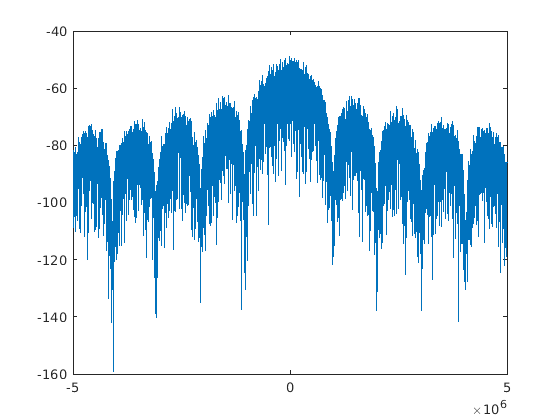
\includegraphics[scale=0.5]{b1}

Compared against the periodograms of the two ideal GNSS signals:

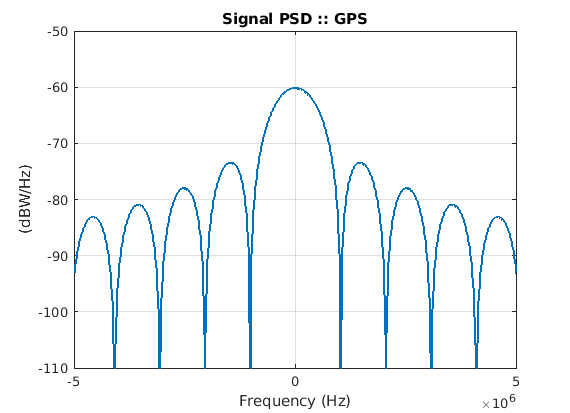
\includegraphics[scale=0.6]{gps}

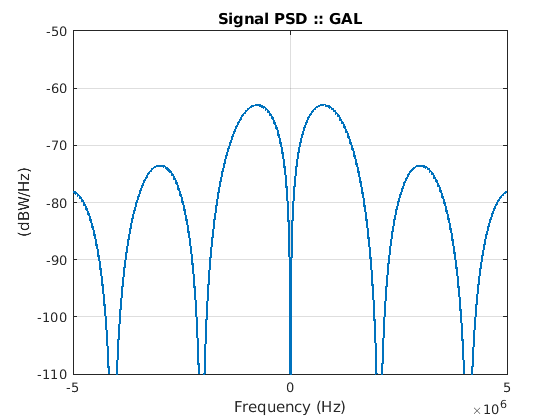
\includegraphics[scale=0.6]{gal}

It's easy to see that our signal is a GPS one, as it has one big lobe at frequency 0. Furthermore if we superpose both graphs we can see that they match:

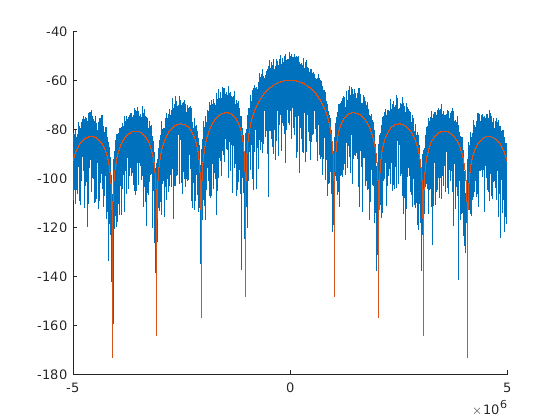
\includegraphics[scale=0.6]{compare}

\section{Bias}
To start our study on the bias present in our calculation let's first do a short analysis on a constant function.

Taking into account equation (1.4) from the practical:
$$E(S^{(per)})=W(e^{jw})*S_x(e^{jw})$$

where $w(m)=1-\frac{|m|}{N}$.

Because the function under study is constant, it's autocorrelation will also be a constant function and the fourier transform of that will be a delta at frequency 0\footnote{This is just a direct consequence of applying the transform}, which means that $S_x(e^{jw})=\delta(e^{jw})$.

Taking this result we can follow the properties of the convolution and we will get that 
$$E(S^{(per)})=W(e^{jw})*\delta(e^{jw})=W(e^{jw})$$

Which means that the estimation of our periodogram will be equal to the fourier transform of $w(m)$.

If our windowing function is a triangle, we could just calculate analytically what's the FT of the triangle function $w$, which would lead us to $sinc^2$. However, instead of doing that we will do calculate it numerically, by plotting the FT of triangle functions of different lengths, to see how that affects our results:

Length 100:

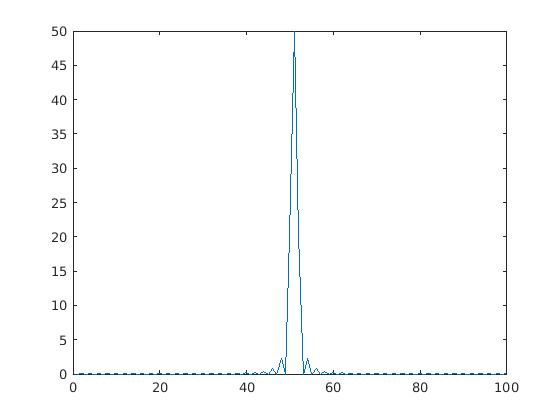
\includegraphics[scale=0.6]{triang100.png}

Length 1000:

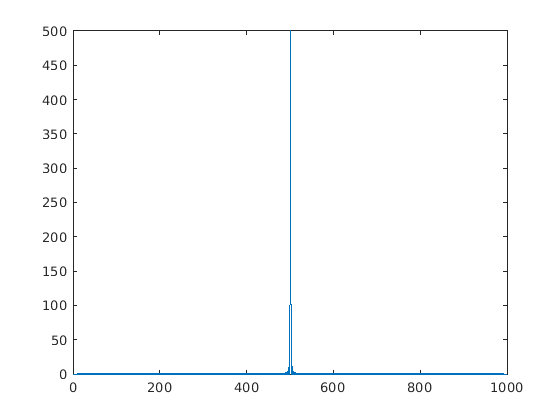
\includegraphics[scale=0.6]{triang1000.png}

As we can see, the higher the length the closer the resulting function is to a delta, with the most power concentrated on frequency 0. This is quite interesting because if the signal that we are manipulating is convoluted by this, in other words, if $W$ takes the form of a delta (which happens at $N=\infty$), the estimated periodogram will unaffected by the convolution and the estimation will be unbiased.

However, because when $N<\infty$ it's not actually a delta and it has non-zero values at frequencies other than zero, the convolution will create shifted copies of the periodogram that will be all summed together to form the estimation\footnote{This is easy to see if we descompose the $sinc^2$ function into a sum of deltas and use the linearity of convolution, as in that case we will end up with a sum of shifted signals}. Practically, this means that in our estimated periodogram we may see values at frequencies where the actual periodogram is zero, a phenomenon called power leakage.

Going back to our signal, our results will be distorted by a multiplication against a triangular function, which means that when we apply the fourier transform we'll se a convolution against $sinc^2$ that shouldn't be there under perfect circustances and adds bias to our result. This corruption of our signals can be attenuated by increasing the amount of samples, which makes the $sinc^2$ function be closer to a delta, the optimal but unachievable situation.

In conclusion, the more samples we use for our estimation, the closer it will be to the real periodogram, as the influence that processes such as power leakage have over the final result will be lowered.

\pagebreak

With that said, we will evaluate how this affects our previous estimates by taking samples of different lengths and comparing several metrics between them.

\subsection{Sample of $50\mu s$ (500 data points)}
Periodogram:

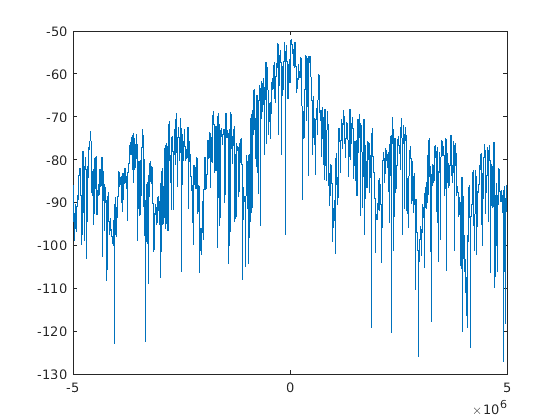
\includegraphics[scale=0.6]{perio500.png}

Error:

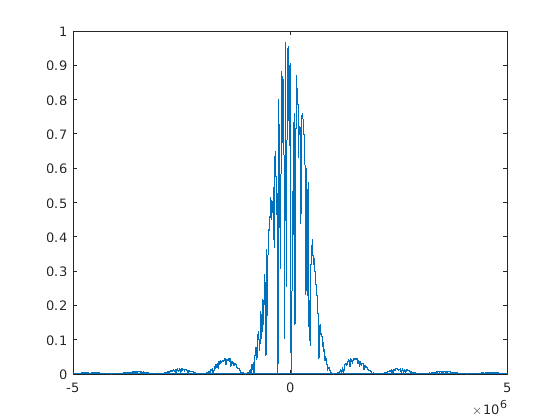
\includegraphics[scale=0.6]{error50.png}

\subsection{Sample of $500\mu s$ (5000 data points)}

Periodogram:

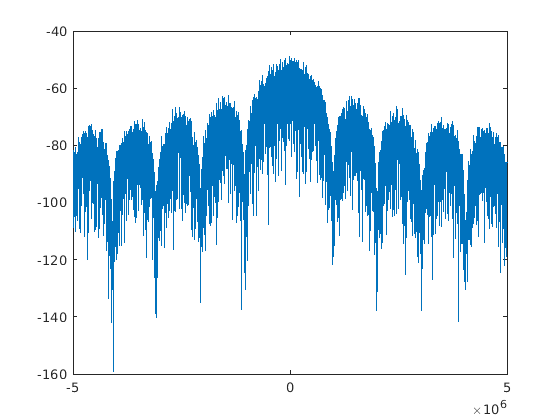
\includegraphics[scale=0.5]{b1}

Error:

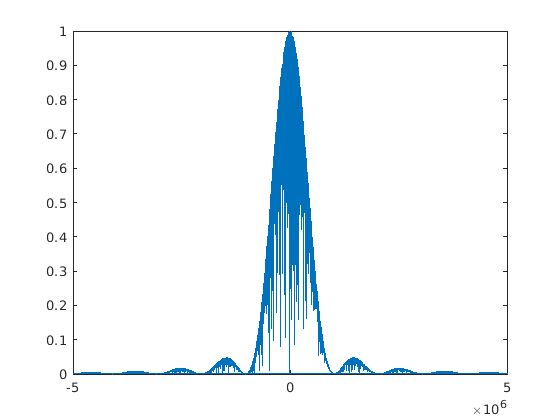
\includegraphics[scale=0.6]{error500.png}

As we can see, the higher the number of samples, the closer the periodogram is to it's real values.

In conclusion, the periodogram is an asymptotically unbiased estimator, since a higher amount of samples gets us a less-biased estimation and when the amount of samples is equal to infinity the bias is gone.

\section{Variance}
In this section we will start delving more into an analysis of the main lobe, which, as we can appreciate in the following plot, is located between -1MHz and 1MHz in the ideal spectrum:

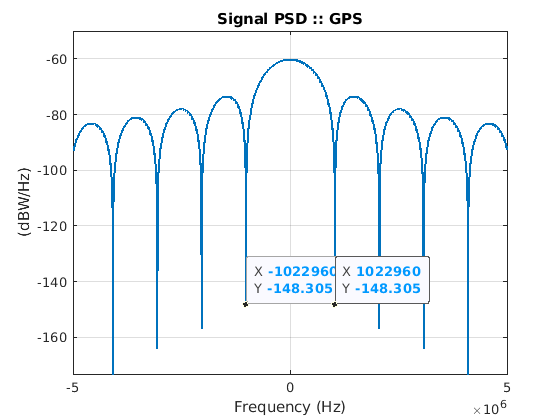
\includegraphics[scale=0.6]{mainlobe.png}

In the beginning of this practical we made sure that the frequncy resolution on which we operate is $10^{-5}$, which means that in total the periodograms that we plot have $10^{5}$ points. As these are distributed evenly in the [-5MHz, 5MHz] frequency range, the point where the main lobe starts will be the $4\cdot 10^4$th, situated at -1MHz, and the point where it ends is the $6\cdot 10^4$th.

Note that this assumes that fftshift has been applied to the result, in case it hasn't, the ranges that hold the main lobe would be [0, 1e4]U[9e4, 1e5].

We can use this now to isolate the errors of our estimation in the main lobe and compute the variance of the resulting vector:

\begin{center}
  \begin{tabular}{ c c }
   N & variance \\ 
   500 &  0.0769 \\  
   5000 & 0.0951    
  \end{tabular}
\end{center}

It seems that variance of the error doesn't change much with the amount of data processed. This means that our estimator is not consistent, as an increase of data points doesn't lead to a decrease in variance.

\section{Bartlett's method}
Next let's test barlett's method, which should get us a lower variance computing the average of multiple periodogram that have been sourced from non-overlapping sections of our signal.

We'll compute various Barlett estimations using different values for L\footnote{See appendix for code}:

\subsection{L=2}
Comparison:

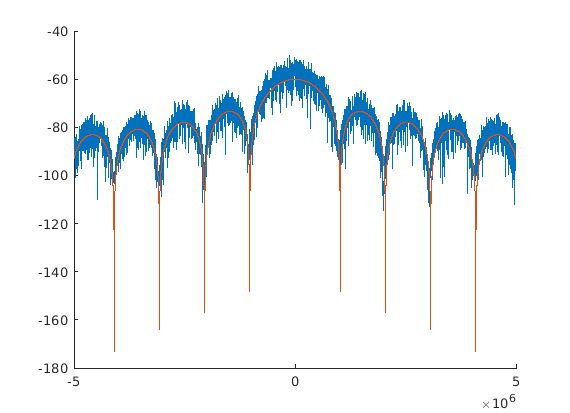
\includegraphics[scale=0.6]{barlett2.png}

Error:

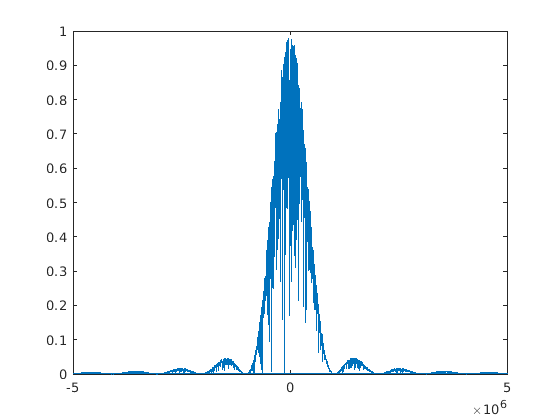
\includegraphics[scale=0.6]{me2.png}

\subsection{L=10}
Comparison:

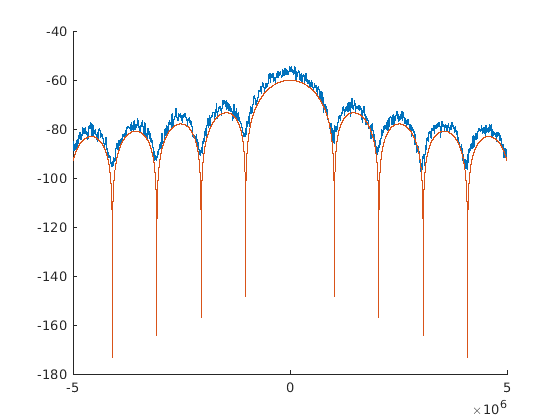
\includegraphics[scale=0.6]{barlett10.png}

Error:

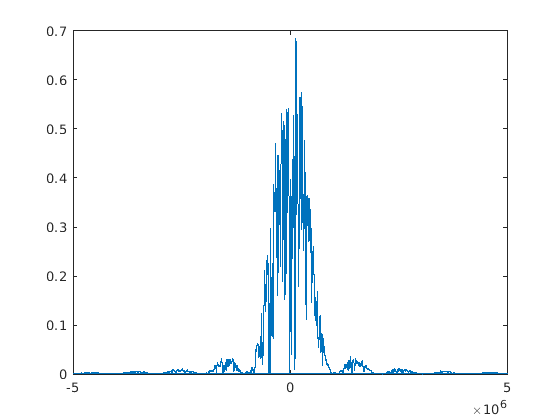
\includegraphics[scale=0.6]{me10.png}

\subsection{L=50}
Comparison:

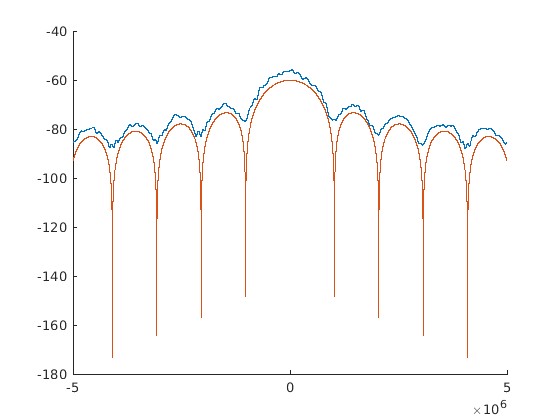
\includegraphics[scale=0.6]{barlett50.png}

Error:

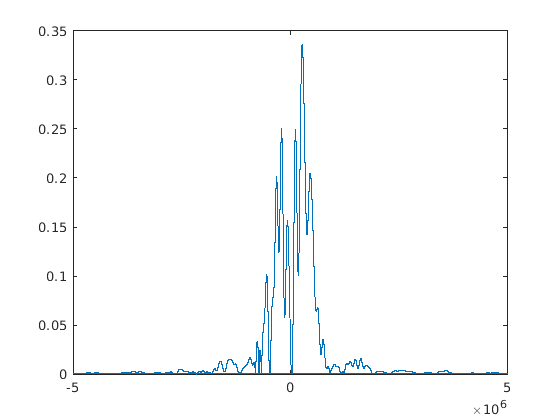
\includegraphics[scale=0.6]{me50.png}

Following our example from before we'll also compute the variance of the error at the main lobe:

\begin{center}
  \begin{tabular}{ c c }
   L & variance \\
   2 &  0.0822 \\
   10 &  0.0275 \\
   50 & 0.0074    
  \end{tabular}
\end{center}

Generally the trend seems to be that the an increase in the value of $L$ causes a decrease of variance at the cost of an increase in the bias (the increase in bias is just observable in plain sight by looking at the decreasing resolution of the results and it's increasing differences against the periodogram of the ideal signal)

% The decrease in bias can be explained by saying that, because now we are averaging multiple estimations of the same value, this average will tend to be closer to the expected value that the estimator provides, and thus the bias will be lower. In other words, averaging a lot of the noise/jitter in the estimation (as seen in previous practicals) and this brings the values closer to the expected ones (the expected values are still biased since we are using a biased estimator here, but that bias is much lower than the error caused by jitter/noise).

The decrese in variance is a direct consequence of the equation (2.1) provided in the practical. An intuitive explanation of this is that by averaging multiple results we get a value closer to the expected one, and as the variance is defined as the squared difference between these, making that smaller causes the variance to get lower aswell.

The increase in bias is caused by the fact that our estimations now use less samples, which decreases the spectral resolution, thus leading to an increase in bias.

\section{AR estimation}
Next we will change our estimator for an AR-based one and see how it responds for different values of p:

\subsection{p=10}
Comparison:

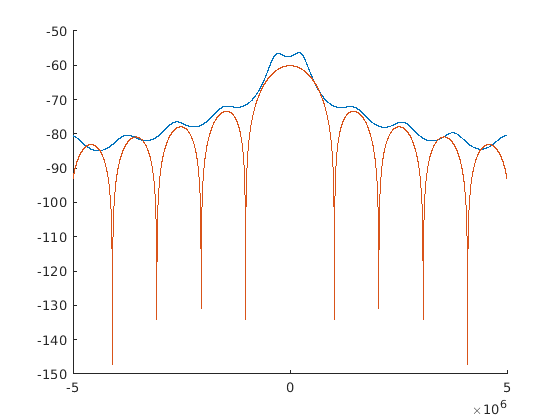
\includegraphics[scale=0.6]{arp10.png}

Error:

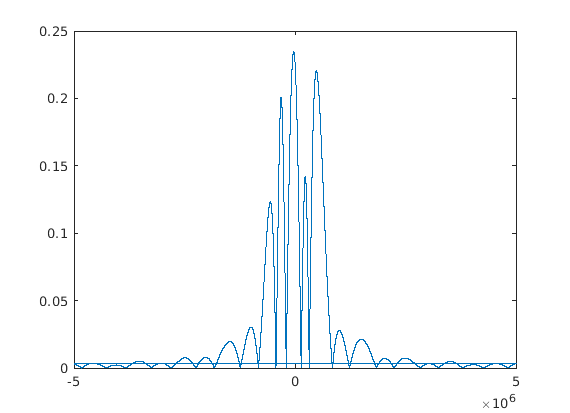
\includegraphics[scale=0.6]{earp10.png}

\subsection{p=100}
Comparison:

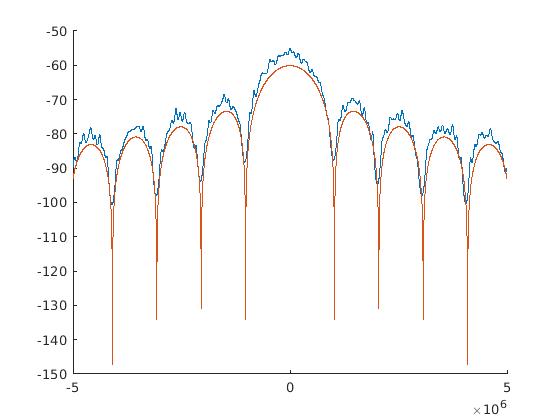
\includegraphics[scale=0.6]{arp100.png}

Error:

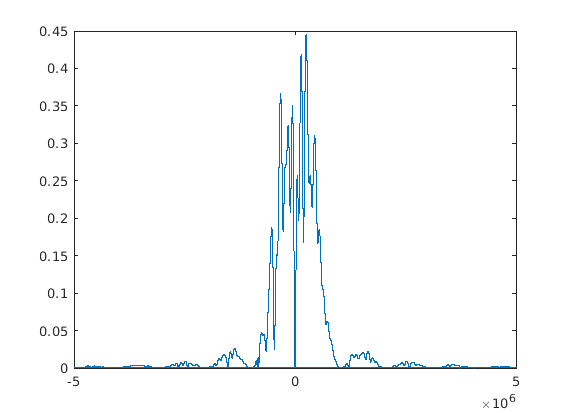
\includegraphics[scale=0.6]{earp100.png}

\subsection{p=1000}
Comparison:

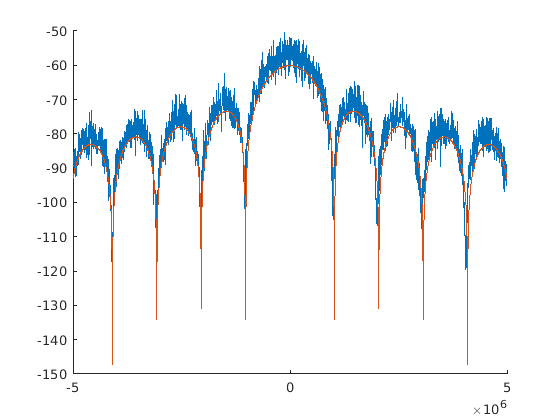
\includegraphics[scale=0.6]{arp1000.png}

Error:

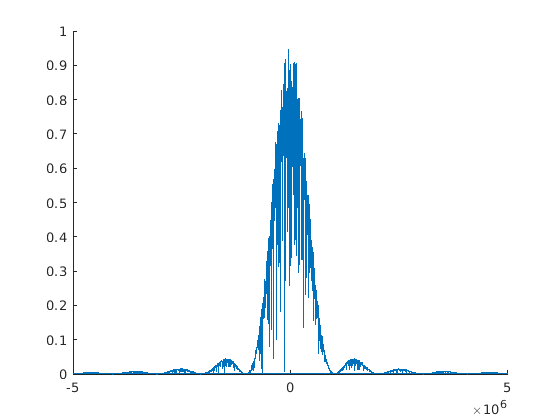
\includegraphics[scale=0.6]{earp1000.png}

As we can appreciate in these graphs, the spectral resolution (and thus the bias) increases with p. This is because when p is low the model that it uses for the signal is simple and it will only be able to fit simple curves, which decreases the frequency resolution (this is also pretty easy to see in the plot of $p=10$, where not many features can be appreciated and only a smooth outline of the result is visible, whereas in the other plots this is no longer the case as the spectral resolution is higher).

In regards to the variance of the errors in the main lobe, we can calculate it using the same code we used previously:

\begin{center}
  \begin{tabular}{ c c }
   p & variance \\
   10 &  0.0051 \\
   100 &  0.0154 \\
   1000 & 0.0805    
  \end{tabular}
\end{center}

It's pretty easy to extrapolate from these results that a higher p results in higher variance. This is because with a higher value of p the model that is being used to simulate the signal gets more complex (since more previous samples are getting used in the estimation of the next one) and therefore the result gets more "wiggly" (if the model is simpler the result is forced to be a simpler function, which makes it smoother and lowers the variance (smoother doesn't directly imply less variance but I'm referring that there's no peaks and sudden changes in the function)).

\section{Conclusion}
In this practical we've analyzed a combined signal, successfully finding out the frequencies of the two signals that made it up through a study of it's power density spectrum, and we've also studied various PDS estimators and applied them to a GNSS signal, analysing the properties that they provide and how they change under different circustances, such as lower amount of samples used.

\section{Appendix}
\subsection{Plot periodogram}
\begin{verbatim}
  N=5000;
  Px=perio(RxSignal(1:N));
  Px=Px.*(max(abs(RxSignal(1:N)))/max(Px));
  x=Fs/N:Fs/N:Fs;
  plot(x, Px)
\end{verbatim}

\subsection{Using peakDetector to detect peaks}
\begin{verbatim}
  for k=[100, 1000, 5000]
    Px=perio(RxSignal(1:k));
    peaks = peakDetector(Px, 2)*10^7/k
  end
\end{verbatim}

\subsection{Plot AR estimations}
\begin{verbatim}
  for p=[10, 100, 1000]
    N=5000;
    Px=compute_AR(RxSignal(1:N), p);
    Px=Px.*(max(abs(RxSignal(1:N)))/max(Px));
    x=Fs/N:Fs/N:Fs;
    plot(x, Px)
  end
\end{verbatim}

\subsection{Log plot}
\begin{verbatim}
function log_plot(S, Fs)
    N=length(S);
    x=-Fs/2:Fs/(N-1):Fs/2;
    y=10*log10(fftshift(S));
    plot(x, y)
end
\end{verbatim}

\subsection{Graphs in first section}
\begin{verbatim}
    log_plot(compute_periodogram(RxSignal), Fs)
    genTruePSD(Fs, 1e5, 'GPS', true)
    genTruePSD(Fs, 1e5, 'GPS', true)
    hold on
    log_plot(compute_periodogram(RxSignal), Fs)
    [f, per] = genTruePSD(Fs, 1e5, 'GPS', false);
    log_plot(per, Fs)
\end{verbatim}

\subsection{Graphs in Bias section}
\begin{verbatim}
  plot(fftshift(abs(fft(triang(100)))))
  plot(fftshift(abs(fft(triang(1000)))))
  log_plot(compute_periodogram(RxSignal(1:100)), Fs)
\end{verbatim}

\subsection{Lineal errors}
\begin{verbatim}
function error=compute_error(est, Fs)
  [f, real] = genTruePSD(Fs, 1e5, 'GPS', false);
  real=real./max(real);
  est=est./max(est);
  error=abs(real-est);
end

est=compute_periodogram(RxSignal(1:5000)); % or 5000
plot(f, error);
\end{verbatim}

\subsection{Compute variance}
\begin{verbatim}
  fe=fftshift(error);
  var(fe(4e4:6e4))
\end{verbatim}

\subsection{Barlett's method}
Using a compute\_periodogram function that uses a same-size FFT:
\begin{verbatim}
function S_per = barlett(signal, L)
  agg=[];
  N=length(signal);
  for c=1:N/L:N
    s=signal(c:c+N/L-1);
    per=compute_periodogram(s);
    agg=[agg; per'];
  end
  S_per=mean(agg);
end
\end{verbatim}

\subsection{Barlett graphs}
\begin{verbatim}
 L=2;
 b=barlett(RxSignal, L);
 [f, real] = genTruePSD(Fs, length(b), 'GPS', false);
 hold on
 plot(f, b)
 plot(f, real)
 % Second plot
 error=compute_error(b', Fs)
 plot(f, error)
\end{verbatim}


\subsection{AR graphs}
\begin{verbatim}
   p=1000
   s=compute_AR(RxSignal, p);
   [f, real] = genTruePSD(Fs, length(s), 'GPS', false);
   hold on
   log_plot(s, Fs)
   log_plot(real, Fs)
   % Second plot
   error=compute_error(s, Fs);
   ferror=fftshift(error);
   var(ferror(4e4:6e4))
   plot(f, error)
\end{verbatim}

\end{document}


